\documentclass[10pt,a4paper]{article}
\usepackage[utf8]{inputenc}
\usepackage[margin=1in]{geometry}
\thispagestyle{empty}

\usepackage{amsmath}
\usepackage{amsfonts}
\usepackage{amssymb}

\usepackage{parskip}

\usepackage{listings}
\usepackage{xcolor}

\usepackage{enumerate}

\usepackage{hyperref}

\usepackage{float}
\usepackage[font=small,labelfont=bf]{caption}
\usepackage{wrapfig}

\usepackage{graphicx}
\restylefloat{figure}

\usepackage{cancel}

\author{Cristian Escudero}
\title{Resumen\\Inteligencia Computacional}
\begin{document}
\maketitle

\begin{verbatim}
[·] Casos de problemas de sobre-aprendizaje.
[·] Importancia de los métodos de error.
[·] Proceso de Validación Cruzada. Problemas si no se hace.
[·] Simplificaciones al realizar Perceptrón Simple.
[·] Deducción fórmula de actualización de pesos Perceptrón Simple activación lineal.
[·] Problemas resueltos por X arquitectura de capas.
[·] Término de momento: inclusión, explicación.
[·] Gradiente de error instantáneo: qué es y qué rol juega.
[·] Fronteras de decisión con perceptrones multicapa base radial.
[$] Etapas de un mapa organizativo: criterios para fijar parámetros.
[·] Mínimos locales: qué son y cómo se evitan.
[·] Etapa de extracción de características: qué es y dar ejemplos reales.
[·] Algoritmo de entrenamiento de una red neuronal con función de base radial. 
Alternativas.
[·] Algoritmo de entrenamiento para una red de Hopfield.
[·] Método de entrenamiento por expansión de una red recurrente y retropropagación.
[·] Análisis comparativo entre los 3 tipos de perceptrones.
[·] Perceptrón multicapa: proceso de retropropagación de forma gráfica,
ecuación general de adaptación para cualquier peso en una capa oculta.
[·] k-medias: forma gráfica, como usarlo para entrenar una red radial.
[·] Hopfield: describir arquitectura, inspiración biológica, particularidades.
[·] Componentes de un sistema de producción con encadenamiento hacia adelante.
[·] Lógica: ¿qué es? ¿para qué sirve? Simántica y sintaxis asociada.
[·] Probabilidad e incerteza: diferencias, ejemplos.
[·] Operador suma disyuntiva: explicación gráfica, definición, ejemplo.
[·] Clasificador estadístico: definición y representación gráfica.
[·] Entropía borrosa: definición y representación gráfica.
[·] Demostración del teorema entropía-subconjunto borroso.
\end{verbatim}

\section*{Introducción (Unidad I)}
\begin{quote}
Breve revisión histórica a la inteligencia computacional. Áreas del conocimiento involucradas y su relación como parte de la inteligencia artificial. El cerebro humano y las limitaciones del cálculo computacional. El impacto y el amplio espectro de aplicaciones de la inteligencia computacional. Introducción conceptual a las tres técnicas fundamentales de la inteligencia computacional.
\end{quote}

\section*{Redes neuronales 1 (Unidad II)}
\begin{quote}
Bases estadísticas del reconocimiento de patrones: etapas, decisión bayesiana, funciones discriminantes. Aprendizaje, espacio de soluciones, mínimos locales y globales, capacidad de generalización y técnicas de validación cruzada. La inspiración biológica en redes neuronales: fisiología neuronal básica, redes de neuronas biológicas y escalas de organización estructural del cerebro. Modelos de neurona: la sinapsis, funciones de activación. Perceptrón simple: hiperplanos para la separación de clases, entrenamiento y limitaciones. Generalidades: características de las redes neuronales, clasificación de las arquitecturas neuronales, clasificación de los procesos de aprendizaje.
\end{quote}

\section*{Redes neuronales 2 (Unidad III)}
\begin{quote}
Perceptrón multicapa: formulación matemática del algoritmo de retropropagación, velocidad de aprendizaje y término de momento, inicialización y criterios de finalización, definición de la topología y los parámetros de entrenamiento. Redes neuronales con funciones de base radial: arquitectura, fronteras de decisión, algoritmos de entrenamiento. Mapas auto-organizativos: arquitecturas, algoritmo de entrenamiento, mapas topológicos, cuantización vectorial con aprendizaje, comparación con otros métodos de agrupamiento. Redes neuronales dinámicas: redes de Hopfield, retropropagación a través del tiempo, redes neuronales con retardos en el tiempo.
\end{quote}

\section*{Lógica borrosa 1 (Unidad IV)}
\begin{quote}
Lógica proposicional: sintaxis, semántica e inferencia. Lógica de primer orden: sintaxis, semántica, cuantificadores y conectores. Inferencia en la lógica de primer orden. Sistemas de producción con encadenamiento hacia delante. La borrosidad como multivalencia: incerteza versus aleatoriedad,  función de membresía. Comparación entre representaciones del conocimiento basadas en reglas. Geometría de los conjuntos borrosos. Definición e interpretación gráfica de los operadores borrosos. Caracterización de conjuntos borrosos. Entropía borrosa: definición, teorema de la entropía borrosa, teorema del subconjunto, teorema entropía-subconjunto.
\end{quote}

\pagebreak

\section{¿Por qué redes neuronales?}

\subsection{Ventajas}
Las \textbf{RNA} tienen muchas ventajas debido a que están basadas en la estructura del sistema nervioso, principalmente el cerebro.
\begin{description}
\item \textbf{Aprendizaje}: Las RNA tienen la habilidad de aprender mediante una etapa que se llama \textit{etapa de aprendizaje}. Esta consiste en proporcionar a la RNA datos como entrada a su vez que se le indica cuál es la salida (respuesta) esperada.
\item \textbf{Auto-organización}: Una RNA crea su propia representación de la información en su interior, descargando al usuario de esto.
\item \textbf{Tolerancia a fallos}: Debido a que una RNA almacena la información de forma redundante, ésta puede seguir respondiendo de manera aceptable aun si se daña parcialmente.
\item \textbf{Flexibilidad}: Una RNA puede manejar cambios no importantes en la información de entrada, como señales con ruido u otros cambios en la entrada.
\item \textbf{Tiempo real}: La estructura de una RNA es paralela, por lo cual si esto es implementado con computadoras o en dispositivos electrónicos especiales, se pueden obtener respuestas en tiempo real.
\end{description}

\subsection{Desventajas}

\begin{itemize}
\item Requieren gran cantidad de datos de entrenamiento diversos para operaciones en el mundo real.
\item Requieren gran tiempo de procesamiento y de memoria.
\end{itemize}

\subsection{Aprendizaje}
El proceso de aprendizaje en un RNA puede ser visto en el contexto de un problema de actualización de la arquitectura y los pesos neuronales en orden de hacer más eficiente a la red para realizar determinada tarea. La habilidad de una RNA de aprender directamente de los ejemplos es la mayor ventaje que tiene frente a los \textbf{sistemas expertos}.

Hay tres paradigmas de aprendizajes principales:
\begin{description}
\item \textbf{Supervisado (\textit{supervised}):} la red es provista de una respuesta correcta (\textit{output}) para cada entrada. Los pesos son determinados en base a permitir a la red producir salidas lo más cercanas a las respuestas correctas.
\subitem \textbf{Aprendizaje reforzado (\textit{reinforcement learning)}:} es una variante del anterior, en el cual la red es provista de sólo una crítica acerca de lo correcto o no que es la salida de la red, no la respuesta correcta de por sí.
\item \textbf{Sin supervisar (\textit{unsupervised}):} no requiere una respuesta correcta asociada con cada entrada en el conjunto de entrenamiento. Explora la estructura interna de la información, y organiza los patrones en categorías en base a las correlaciones entre ellos.
\item \textbf{Híbrido (\textit{hybrid}):} una parte de los pesos son determinados a traves de un entrenamiento \textbf{\textit{supervisado}}, y el resto son obtenidos a través de un aprendizaje \textbf{\textit{sin supervisar}}.
\end{description}

\subsection{Reglas de Aprendizaje}
\subsubsection{Corrección de Error}
Es la que utiliza el \textbf{perceptrón}. Su principio básico es el de usar la señal de error ($y_{\text{deseado}}-y$) para modificar los pesos para gradualmente ir reduciendo el error. El aprendizaje sólo ocurre cuando se comete un error.

\begin{quotation}
\textit{Perceptron Convergence Theorem:} si los patrones se ubican en dos clases linealmente separables, el procedimiento de aprendizaje del perceptrón converge luego de un número finito de iteraciones, siempre y cuando se utilice una \textbf{función de activación} monótona.
\end{quotation}

\subsubsection{Boltzmann}
Un subconjunto de neuronas llamadas \textbf{visibles} interactúan con el entorno; el resto, llamadas \textbf{ocultas} (\textit{hidden}), no. El objetivo es ajustar los pesos sinápticos para que el estado de las neuronas visibles satisfagan una distribución de probabilidad deseada.

\subsubsection{Hebbiano}
Es la regla más antigüa. Si las neuronas en ambos lados de la sinapsis son actividas sincronizadamente y repetitivamente, la fuerza sináptica es incrementada de forma selectiva. Matemáticamente:
\[w_{ij}(t+1) = w_{ij}(t) + \eta \: y_j(t)x_i(t),\]
dónde $x_i$ e $y_j$ son las salidas de las neuronas $i$ y $j$ respectivamente, conectadas por la sinapsis $w_{ij}$.

El aprendizaje es hecho de forma local: el cambio en los pesos sinápticos depende sólo de las actividades de las dos neuronas conectadas por él.

\subsubsection{Competitivo}
Las unidades de salida compiten entre sí para ver cuál se activa. Como resultado, sólo una se activa en un cierto tiempo: \textbf{el ganador se lo lleva todo} (\textit{winner-take-all}). 

Normalmente categorizan la información de entrada, agrupando automáticamente patrones similares basándose en las correlaciones entre ellos.

\begin{quotation}
\textit{Stability-Plasticity Dilemma}: un sistema de aprendizaje es \textit{estable} si ningún patrón dentro del conjunto de entrenamiento cambia de categoría luego de un número finitio de iteraciones. Esto puede lograrse forzando a la $\eta$ a decrecer gradualmente a cero. Pero esto causa otro problema conocido como \textit{plasticibilidad}, que es la habilidad de adaptarse a la nueva información. De ahí el dilema en el aprendizaje competitivo.
\end{quotation}

\subsection{Validación Cruzada}

La validación cruzada o cross-validation es una técnica utilizada para evaluar los resultados de un análisis estadístico y garantizar que son independientes de la partición entre datos de entrenamiento y prueba. Consiste en repetir y calcular la media aritmética obtenida de las medidas de evaluación sobre diferentes particiones. Se utiliza en entornos donde el objetivo principal es la predicción y se quiere estimar cómo de preciso es un modelo que se llevará a cabo a la práctica. Es una técnica muy utilizada en proyectos de inteligencia artificial para validar modelos generados.

\subsubsection{Contexto}
La validación cruzada proviene de la mejora del método de retención o holdout method. Este consiste en dividir en dos conjuntos complementarios los datos de muestra, realizar el análisis de un subconjunto (denominado datos de entrenamiento o training set), y validar el análisis en el otro subconjunto (denominado datos de prueba o test set), de forma que la función de aproximación sólo se ajusta con el conjunto de datos de entrenamiento y a partir de aquí calcula los valores de salida para el conjunto de datos de prueba (valores que no ha analizado antes). La ventaja de este método es que es muy rápido a la hora de computar. Sin embargo, este método no es demasiado preciso debido a la variación del resultados obtenidos para diferentes datos de entrenamiento. La evaluación puede depender en gran medida de cómo es la división entre datos de entrenamiento y de prueba, y por lo tanto puede ser significativamente diferente en función de cómo se realice esta división. Debido a estas carencias aparece el concepto de validación cruzada.

\subsubsection{Objetivos}
Suponemos que tenemos un modelo con uno o más parámetros de ajuste desconocidos y unos datos de entrenamiento que queremos analizar. El proceso de ajuste optimiza los parámetros del modelo para que éste se ajuste a los datos de entrenamiento tan bien como pueda. Si cogemos una muestra independiente como dato de prueba (validación), del mismo grupo que los datos de entrenamiento, normalmente el modelo no se ajustará a los datos de prueba igual de bien que a los datos de entrenamiento. Esto se denomina sobreajuste y acostumbra a pasar cuando el tamaño de los datos de entrenamiento es pequeño o cuando el número de parámetros del modelo es grande. La validación cruzada es una manera de predecir el ajuste de un modelo a un hipotético conjunto de datos de prueba cuando no disponemos del conjunto explícito de datos de prueba.

\subsubsection{Limitaciones y uso no adecuado}
La validación cruzada sólo produce resultados significativos si el conjunto de validación y prueba de conjunto se han extraído de la misma población. En muchas aplicaciones de modelado predictivo, la estructura del sistema que está siendo estudiado evoluciona con el tiempo. Esto puede introducir diferencias sistemáticas entre los conjuntos de entrenamiento y validación. Por ejemplo, si un modelo para predecir el valor de las acciones está entrenado con los datos de un período de cinco años determinado, no es realista para tratar el siguiente período de cinco años como predictor de la misma población.

Otro ejemplo, supongamos que se desarrolla un modelo para predecir el riesgo de un individuo para ser diagnosticado con una enfermedad en particular en el próximo año. Si el modelo se entrena con datos de un estudio que sólo afecten a un grupo poblacional específico (por ejemplo, solo jóvenes o solo hombres varones), pero se aplica luego a la población en general, los resultados de la validación cruzada del conjunto de entrenamiento podrían diferir en gran medida de la clasificación real.

Si se lleva a cabo correctamente, y si el conjunto de validación y de conjunto de entrenamiento son de la misma población, la validación cruzada es casi imparcial. Sin embargo, hay muchas maneras en que la validación cruzada puede ser mal utilizada. Si se abusa y posteriormente se lleva a cabo un estudio real de validación, es probable que los errores de predicción en la validación real sean mucho peores de lo esperado sobre la base de los resultados de la validación cruzada.

Estas son algunas formas en que la validación cruzada puede ser mal utilizada:

* Mediante el uso de la validación cruzada para evaluar varios modelos, y sólo indicando los resultados para el modelo con los mejores resultados.

* Al realizar un análisis inicial para identificar las características más informativas utilizando el conjunto de datos completo, si la selección de característica o el ajuste del modelo lo requiere por el propio procedimiento de modelado, esto debe repetirse en cada conjunto de entrenamiento. Si se utiliza la validación cruzada para decidir qué características se van a utilizar, se deberá realizar un proceso interno de validación cruzada para llevar a cabo la selección de características en cada conjunto de entrenamiento.

* Al permitir que algunos de los datos de entrenamiento esté también incluido en el conjunto de prueba, esto puede suceder debido a "hermanamiento" en el conjunto de datos, con lo que varias muestras exactamente idénticas o casi idénticas pueden estar presentes en el conjunto de datos.

\subsection{Aplicaciones de las RNA}
Las características de las \textbf{RNA} las hacen bastante apropiadas para aplicaciones en las que no se dispone a priori de un modelo identificable que pueda ser programado, pero se dispone de un conjunto básico de ejemplos de entrada (previamente clasificados o no). Asimismo, son altamente robustas tanto al ruido como a la disfunción de elementos concretos y son fácilmente paralelizables.

Esto incluye problemas de clasificación y reconocimiento de patrones de voz, imágenes, señales, etc. Asimismo se han utilizado para encontrar patrones de fraude económico, hacer predicciones en el mercado financiero, hacer predicciones de tiempo atmosférico, etc.

También se pueden utilizar cuando no existen modelos matemáticos precisos o algoritmos con complejidad razonable.

\section{Perceptrón Simple}

\section{Perceptrón Multicapa}

\begin{figure}[h!]
  \caption{Interpretación geométrica del rol de las neuronas ocultas en un espacio de dos entradas.}
  \label{fig:layers}
  \centering
  \hbox{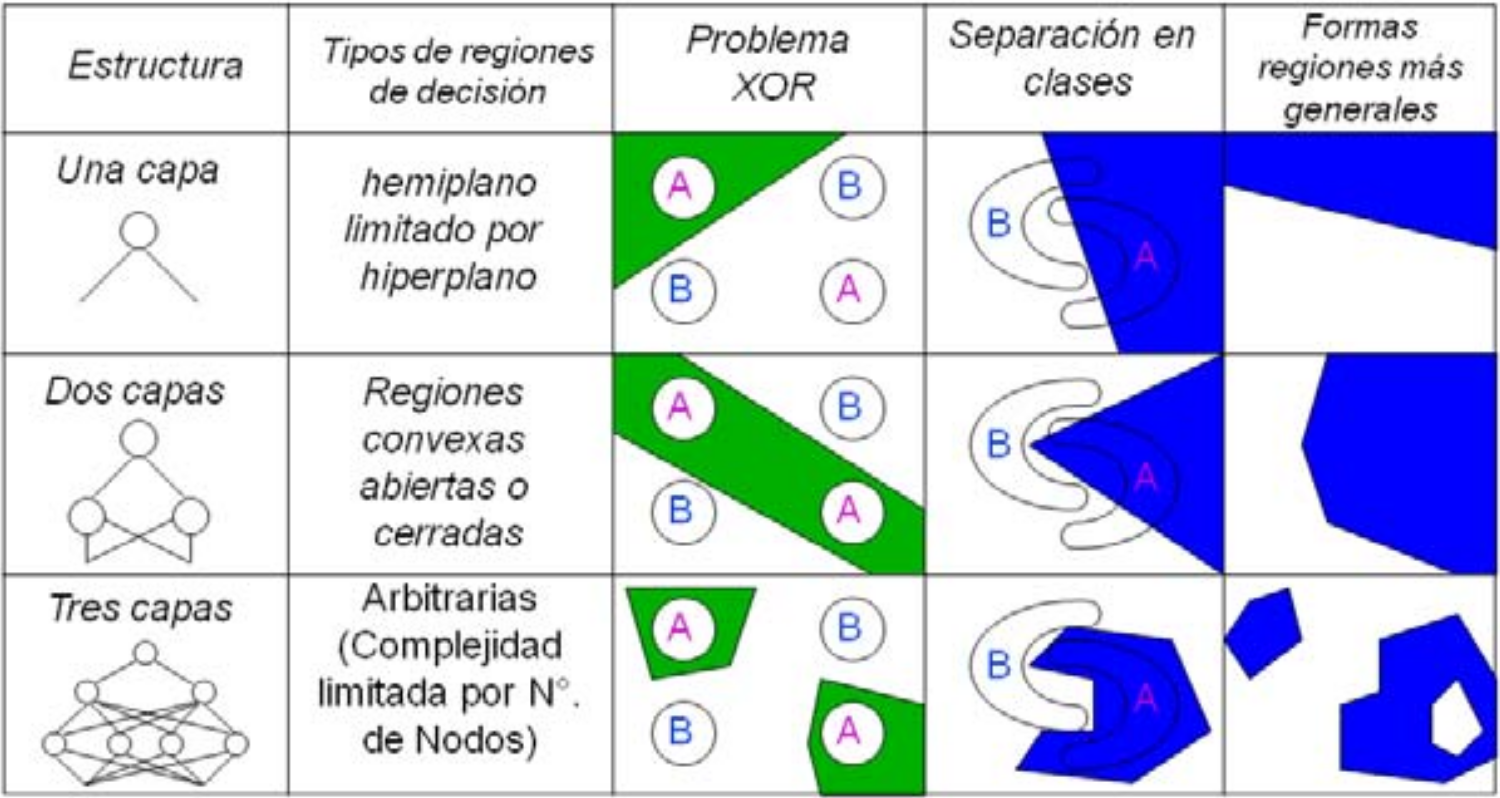
\includegraphics[width=\textwidth-\fboxrule-\fboxrule]{layers.png}}
\end{figure}

\section{Mapas Auto-Organizativos (SOM)}

Este tipo de red está basada en el aprendizaje \textit{competitivo}; las neuronas de salida de la red compiten entre ellas para ver cual será activada, dando como resultado que una sóla neurona, o neurona por grupo, es activada a la vez (\textit{winner takes all}).

Las neuronas son ubicadas...

\subsection{Etapas de Entrenamiento}
\begin{description}
\item \textbf{Ordenamiento.} Durante esta primera fase es donde el proceso adaptativo  del ordenamiento topológico de los vectores de pesos toma lugar. Puede llegar a tomar 1000 iteraciones del algoritmo de SOM o más.
\subitem \textbf{Tasa de aprendizaje:} debe permanecer desde el inicio con un valor cercano a 0.1; decreciendo gradualmente pero permaneciendo sobre 0.01.
\subitem \textbf{Función vecindad $h_{j,i} (n)$:} debe inicialmente incluir a todas las neuronas en la red, centrado en la neurona ganadora $i$, e ir cubriendo menos a lo largo del tiempo.
\item \textbf{Convergencia.} Esta segunda fase es necesaria para hacer un ajuste fino de los datos y obtener de esa manera una cuantificación estadística adecuada. Como regla general, se requieren 500 iteraciones por el número de neuronas.
\subitem \textbf{Tasa de aprendizaje:} debe mantenerse en un valor bajo, del orden de $0.01$, sin nunca llegar a cero.
\subitem \textbf{Función vecindad $h_{j,i} (n)$:} debe contener solamente a las neuronas más cercanas a la ganadora, o incluso llegar a contener solamente a la ganadora.
\end{description}

\section{Lógica Borrosa}

\pagebreak

\section{Abreviaciones}
\begin{itemize}
\item \textbf{RNA}: Redes Neuronales Artificiales.
\end{itemize}

\section{Bibliografía}
\begin{description}
\item Artificial Neuronal Networks: A Tutorial.
\item Wikipedia
\end{description}

\end{document}